\subsection{Exercise 4.1: Quicksort Partitioning Worst Case}
\textbf{Problem:} Prove that the worst case in Partitioning Algorithm (for Quicksort) has running time $\Theta(n^2)$, where $n$ is the cardinality of the set of elements in the partitioning.

\textbf{Solution:} We provide both an intuitive proof and a formal proof by induction.

\textbf{Part 1: Intuitive Proof}
\begin{enumerate}[leftmargin=*,noitemsep]
    \item \textbf{Worst Case Scenario:}
    \begin{itemize}[noitemsep]
        \item At each step, we get maximally unbalanced partitions:
        \item A $k-1$ element array and an empty array
        \item This happens when pivot is always smallest/largest element
    \end{itemize}

    \item \textbf{Recurrence Relation:}
    Let $T(n)$ be the running time of Quicksort with Partition:
    \begin{itemize}[noitemsep]
        \item Splitting time is linear: $\Theta(k)$ for array of size $k$
        \item Base case: $T(0)$ is constant, so $T(0) = \Theta(1)$
        \item For size $k$: $T(k) = T(k-1) + T(0) + \Theta(k)$
        \item Simplifies to: $T(k) = T(k-1) + \Theta(k)$
    \end{itemize}

    \item \textbf{Solving the Recurrence:}
    \begin{align*}
        T(n) &= T(n-1) + \Theta(n) \\
        &= T(n-2) + \Theta(n-1) + \Theta(n) \\
        &= T(n-3) + \Theta(n-2) + \Theta(n-1) + \Theta(n) \\
        &\vdots \\
        &= T(0) + \sum_{i=1}^n \Theta(i)
    \end{align*}

    \item \textbf{Final Step:}
    \begin{itemize}[noitemsep]
        \item Sum is arithmetic series: $\sum_{i=1}^n i$
        \item Using identity: $\sum_{i=1}^n i = \frac{n(n+1)}{2}$
        \item Therefore: $T(n) = \Theta(n^2)$
    \end{itemize}
\end{enumerate}

\textbf{Part 2: Formal Proof by Induction}
\begin{enumerate}[leftmargin=*,noitemsep]
    \item \textbf{Claim:} $T(n) = \Theta(n^2)$ for worst-case running time
    
    \item \textbf{Precise Statement:}
    \begin{itemize}[noitemsep]
        \item For all $0 < m < n$: $T(m) = \Theta(m^2)$
        \item This means $\exists c_1,d_1 > 0: c_1m^2 \leq T(m) \leq d_1m^2$
        \item Partition time $P(m) = \Theta(m)$, so $\exists c_2,d_2 > 0: c_2m \leq P(m) + T(0) \leq d_2m$
    \end{itemize}

    \item \textbf{Constants:}
    \begin{itemize}[noitemsep]
        \item Let $c = \min\{c_1,c_2\}$ and $d = \max\{d_1,d_2,1\}$
        \item Then for all $m \geq n-1$: $cm^2 \leq T(m) \leq dm^2$
        \item And for all $m \geq n$: $2cm \leq T(0) + P(m) \leq dm$
    \end{itemize}

    \item \textbf{Inductive Step:}
    \begin{align*}
        T(n) &= T(n-1) + T(0) + P(n) \\
        c(n-1)^2 + 2cn &\leq cn^2 - 2cn + 1 + 2cn = cn^2 + 1 \\
        d(n-1)^2 + dn &\leq dn^2 - dn + 1 \leq dn^2
    \end{align*}

    Therefore: $cn^2 < T(n) \leq dn^2$, proving $T(n) = \Theta(n^2)$
\end{enumerate}

\textbf{Key Insights:}
\begin{itemize}[noitemsep]
    \item The worst case occurs with extremely unbalanced partitions
    \item Each partition step costs linear time
    \item The cumulative effect leads to quadratic runtime
    \item Both intuitive and formal proofs confirm $\Theta(n^2)$ complexity
\end{itemize}

\subsection{Exercise 4.2: COUNTING-SORT Algorithm}
\textbf{Problem:} We apply COUNTING-SORT with the input vector $A = (5,6,5,3,3,7,4,4,4,5,3,8,8)$. Let $C$ and $B$ be the arrays mentioned in the pseudocode of COUNTING-SORT. Answer the following questions:

\begin{enumerate}[leftmargin=*,noitemsep]
    \item What is $C[7]$ after the for loop at lines 7-8 of the pseudocode?
    \item What is $B[13]$ after the first cycle at line 10?
    \item What is $C[8]$ after the first cycle?
\end{enumerate}

\textbf{Solution:} Let's solve this step by step following the COUNTING-SORT algorithm.

\textbf{1. Algorithm Overview:}
\begin{itemize}[noitemsep]
    \item Input array $A = (5,6,5,3,3,7,4,4,4,5,3,8,8)$ with $k=8$ (max value)
    \item Array $C[0..k]$ is used for counting and cumulative sums
    \item Array $B[1..n]$ will store the sorted output
\end{itemize}

\textbf{2. Step-by-Step Execution:}
\begin{enumerate}[leftmargin=*,noitemsep]
    \item \textbf{Initialize array $C$:}
    \begin{itemize}[noitemsep]
        \item Create $C[0..8]$ initialized to zeros
        \item $C = [0,0,0,0,0,0,0,0,0]$
    \end{itemize}

    \item \textbf{Count elements (lines 3-4):}
    \begin{itemize}[noitemsep]
        \item Count occurrences of each value in $A$
        \item After this step: $C = [0,0,0,3,3,3,1,1,2]$
        \item Meaning: three 3s, three 4s, three 5s, one 6, one 7, two 8s
    \end{itemize}

    \item \textbf{Compute cumulative sums (lines 5-6):}
    \begin{itemize}[noitemsep]
        \item Transform $C$ into cumulative counts
        \item $C = [0,0,0,3,6,9,10,11,13]$
        \item Therefore, $C[7] = 11$ (\textbf{Answer to Question 1})
    \end{itemize}

    \item \textbf{Build sorted array (lines 7-8):}
    \begin{itemize}[noitemsep]
        \item Process $A$ from right to left
        \item Place elements in $B$ based on $C$ values
        \item After first cycle (processing last element 8):
            \begin{itemize}[noitemsep]
                \item $B[13] = 8$ (\textbf{Answer to Question 2})
                \item $C[8]$ is decremented to 12 (\textbf{Answer to Question 3})
            \end{itemize}
        \item Final sorted array: $B = [3,3,3,4,4,4,5,5,5,6,7,8,8]$
    \end{itemize}
\end{enumerate}

\textbf{Key Insights:}
\begin{itemize}[noitemsep]
    \item The cumulative sum array $C$ helps maintain stability by tracking positions
    \item Processing from right to left ensures stability
    \item $C[i]$ represents the position after which the next element $i$ should be placed
    \item Each placement decrements the corresponding counter in $C$
\end{itemize}

\textbf{Final Answers:}
\begin{enumerate}[noitemsep]
    \item $C[7] = 11$
    \item $B[13] = 8$
    \item $C[8] = 12$
\end{enumerate}

\subsection{Exercise 5.1: BUILDKDTREE Algorithm}
\textbf{Problem:} We apply BUILDKDTREE$(P,0)$ to the following set $P$ of points in the plane:
\[ P = \{(1,3), (12,1), (4,5), (5,4), (10,11), (8,2), (2,7)\} \]

Answer the following questions:
\begin{enumerate}[leftmargin=*,noitemsep]
    \item Give the height of the tree
    \item How many leaves are there?
    \item The second leaf (starting from left) is the point with first coordinate...
\end{enumerate}

\textbf{Solution:} Let's solve this step by step following the BUILDKDTREE algorithm.

\textbf{1. Algorithm Review:}
\begin{itemize}[noitemsep]
    \item At even depths (0,2,...): split on x-coordinate (vertical line)
    \item At odd depths (1,3,...): split on y-coordinate (horizontal line)
    \item Each split creates a new level in the tree
    \item Points are recursively divided into left and right subsets
\end{itemize}

\textbf{2. Step-by-Step Construction:}
\begin{enumerate}[leftmargin=*,noitemsep]
    \item \textbf{Root Level (depth 0, x-split):}
    \begin{itemize}[noitemsep]
        \item Sort by x-coordinate: $(1,3), (2,7), (4,5), (5,4), (8,2), (10,11), (12,1)$
        \item Median point $(5,4)$ becomes root $\ell_1$
        \item Left subset: $\{(1,3), (2,7), (4,5)\}$
        \item Right subset: $\{(8,2), (10,11), (12,1)\}$
    \end{itemize}

    \item \textbf{Level 1 (depth 1, y-split):}
    \begin{itemize}[noitemsep]
        \item Left subset sorted by y: $(1,3), (4,5), (2,7)$
        \item Right subset sorted by y: $(12,1), (8,2), (10,11)$
        \item Medians $(2,7)$ and $(10,11)$ become nodes $\ell_2$ and $\ell_3$
    \end{itemize}

    \item \textbf{Level 2 (depth 2, x-split):}
    \begin{itemize}[noitemsep]
        \item Split remaining points into leaf nodes
        \item Left of $\ell_2$: $(1,3), (4,5)$ become leaves under $\ell_4$
        \item Left of $\ell_3$: $(8,2), (12,1)$ become leaves under $\ell_6$
    \end{itemize}
\end{enumerate}

\begin{figure}[H]
    \centering
    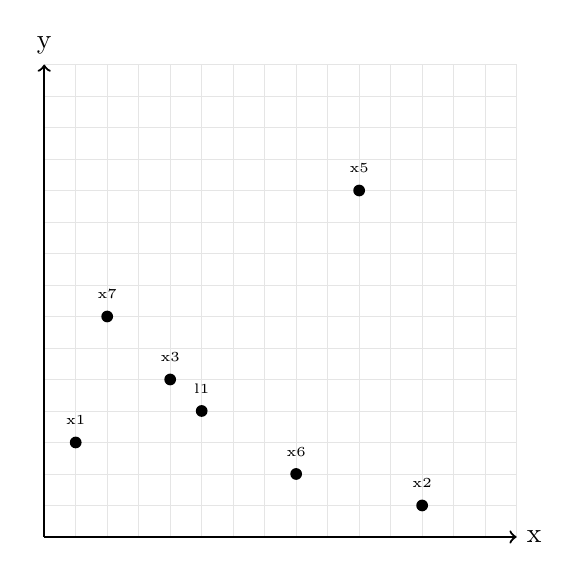
\begin{tikzpicture}[scale=0.4]
        % Grid
        \draw[very thin,gray!20] (0,0) grid (15,15);
        \draw[->,thick] (0,0) -- (15,0) node[right] {x};
        \draw[->,thick] (0,0) -- (0,15) node[above] {y};
        
        % Points with labels
        \node[circle,fill,inner sep=1.5pt] (x1) at (1,3) {};
        \node[font=\tiny] at (1,3.7) {x1};
        
        \node[circle,fill,inner sep=1.5pt] (x2) at (12,1) {};
        \node[font=\tiny] at (12,1.7) {x2};
        
        \node[circle,fill,inner sep=1.5pt] (x3) at (4,5) {};
        \node[font=\tiny] at (4,5.7) {x3};
        
        \node[circle,fill,inner sep=1.5pt] (x4) at (5,4) {};
        \node[font=\tiny] at (5,4.7) {l1};
        
        \node[circle,fill,inner sep=1.5pt] (x5) at (10,11) {};
        \node[font=\tiny] at (10,11.7) {x5};
        
        \node[circle,fill,inner sep=1.5pt] (x6) at (8,2) {};
        \node[font=\tiny] at (8,2.7) {x6};
        
        \node[circle,fill,inner sep=1.5pt] (x7) at (2,7) {};
        \node[font=\tiny] at (2,7.7) {x7};
    \end{tikzpicture}
    \caption*{Points in 2D plane}
\end{figure}

\begin{figure}[H]
    \centering
    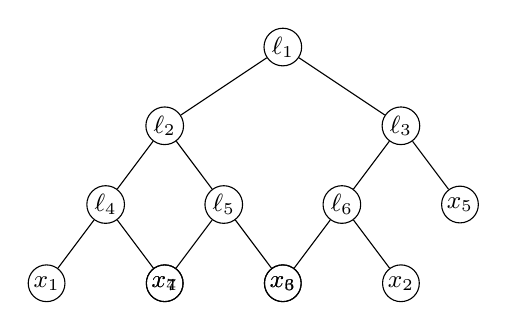
\begin{tikzpicture}[
        level distance=1cm,
        level 1/.style={sibling distance=3cm},
        level 2/.style={sibling distance=1.5cm},
        every node/.style={circle,draw,inner sep=1pt,font=\small}
    ]
        \node {$\ell_1$}
            child {node {$\ell_2$}
                child {node {$\ell_4$}
                    child {node {$x_1$}}
                    child {node {$x_4$}}
                }
                child {node {$\ell_5$}
                    child {node {$x_7$}}
                    child {node {$x_3$}}
                }
            }
            child {node {$\ell_3$}
                child {node {$\ell_6$}
                    child {node {$x_6$}}
                    child {node {$x_2$}}
                }
                child {node {$x_5$}}
            };
    \end{tikzpicture}
    \caption*{Final KD-Tree structure}
\end{figure}

\textbf{3. Answers:}
\begin{enumerate}[noitemsep]
    \item Height of the tree = 3 (counting levels from 0)
    \item Number of leaves = 7 (each original point becomes a leaf)
    \item Second leaf from left = $x_4 = (4,5)$
\end{enumerate}

\textbf{Key Insights:}
\begin{itemize}[noitemsep]
    \item The tree is built by alternating between x and y coordinates
    \item Each internal node represents a splitting line
    \item Vertical splits (even depths) compare x-coordinates
    \item Horizontal splits (odd depths) compare y-coordinates
    \item All original points end up as leaves
\end{itemize}

\subsection{Exercise 5.2: BUILDKDTREE Complexity}
\textbf{Problem:} (It is enough to give an intuitive idea) Prove that the BUILDKDTREE for a set of $n$ points has running time $O(n \log n)$ and uses $O(n)$ storage.

\textbf{Solution:} Let's break this down into two parts: storage complexity and runtime complexity.

\textbf{1. Storage Complexity $O(n)$:}
\begin{itemize}[noitemsep]
    \item Each splitting line divides points into two equal parts (up to unity)
    \item For $n = 2^k$ points, we need $2^k - 1$ lines (internal nodes)
    \item For splitting 2, the total nodes (parents + leaves) is:
        \[ 2^k + 2^{k-1} = n + n/2 = 3n/2 < 3n \]
    \item For $n$ not a power of 2, there exists $t$ where $2^{t-1} < n < 2^t$
    \item Number of internal nodes $n_p$ is bounded by:
        \[ 2^{t-2} < n_p < 2^{t-1} \]
    \item Total nodes (parents + leaves) satisfies:
        \[ 3 \cdot 2^{t-2} < n + n_p < 3 \cdot 2^{t-1} \]
    \item Therefore: $n + n_p < 3 \cdot 2^{t-1} < 3n$
    \item Each node uses $O(1)$ storage
    \item Total storage: $O(1) \cdot O(n) = O(n)$
\end{itemize}

\textbf{2. Runtime Complexity $O(n \log n)$:}
\begin{itemize}[noitemsep]
    \item BUILDKDTREE is recursive:
        \begin{itemize}[noitemsep]
            \item Each recursion splits $n$ points into two $n/2$ subsets
            \item Split cost is linear ($O(n)$): finding median in x or y coordinates
        \end{itemize}
    \item Building time $T(n)$ follows the recurrence:
        \[ T(n) = \begin{cases}
            O(1) & \text{if } n = 1 \\
            2T(n/2) + O(n) & \text{if } n > 1
        \end{cases} \]
    \item By Master Theorem (as in Merge-Sort):
        \begin{itemize}[noitemsep]
            \item $a = 2$ (subproblems)
            \item $b = 2$ (size reduction)
            \item $f(n) = O(n)$ (split cost)
            \item Case 1: $f(n) = O(n) = \Theta(n^{\log_2 2}) = \Theta(n)$
            \item Therefore: $T(n) = O(n \log n)$
        \end{itemize}
\end{itemize}

\textbf{Key Insights:}
\begin{itemize}[noitemsep]
    \item Storage is linear because each point becomes exactly one leaf node
    \item Runtime is $O(n \log n)$ due to:
        \begin{itemize}[noitemsep]
            \item Linear-time splitting at each level
            \item Logarithmic number of levels in the tree
        \end{itemize}
\end{itemize}

\begin{itemize}
    \item Example of a point $p_1$ \hfill
\end{itemize}

\begin{itemize}
    \item Example of a point $p_2$ \hfill
\end{itemize}

\begin{itemize}
    \item Example of a point $p_3$ \hfill
\end{itemize}

\begin{itemize}
    \item Example of a point $p_4$ \hfill
\end{itemize}

\begin{itemize}
    \item Example of a point $p_5$ \hfill
\end{itemize}
